\documentclass{article}
\usepackage[utf8]{inputenc}  
\usepackage[T1]{fontenc}     
\usepackage{tikz}
\usetikzlibrary{shapes,positioning,arrows,calc}

\begin{document}

% file : exemple


\begin{tikzpicture}[queue/.style={fill=blue!20, font=\sffamily\Large\bfseries, rectangle split, rectangle split parts=5, rectangle split horizontal, draw, anchor=center}]

\node [queue] (queue)  {$13$\nodepart{two}$-1$%
   \nodepart{three}$42$\nodepart{four}$80$\nodepart{five}$1$};
\node [above right=-0.05cm and 1.3cm of queue,anchor=north,align=left] {Début de la file};
\node [above left=-0.05cm and 1.3cm of queue,anchor=north,align=left] {Fin de la file};

\end{tikzpicture}

% file : exemple ajout

\vspace{3cm}
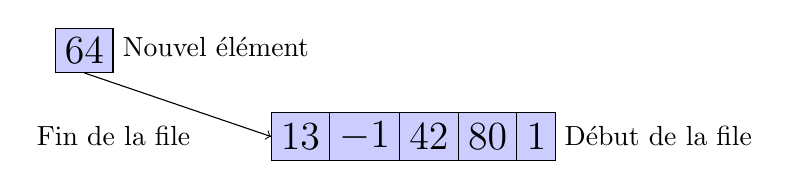
\begin{tikzpicture}[queue/.style={fill=blue!20, font=\sffamily\Large\bfseries, rectangle split, rectangle split parts=5, rectangle split horizontal, draw, anchor=center}, new/.style={fill=blue!20, font=\sffamily\Large\bfseries, rectangle, draw, anchor=center}]

\node [queue] (queue)  {$13$\nodepart{two}$-1$%
   \nodepart{three}$42$\nodepart{four}$80$\nodepart{five}$1$};
\node [above right=-0.05cm and 1.3cm of queue,anchor=north,align=left] {Début de la file};
\node [above left=-0.05cm and 2cm of queue,anchor=north,align=left] {Fin de la file};

\node [new,above left=0.5cm and 2cm of queue] (n) {$64$};
\node [above right=0cm and 1.3cm of n,anchor=north,align=left] {Nouvel élément};
\draw [->] (n.south)--(queue.west);

\end{tikzpicture}


% file : exemple suppression

\vspace{3cm}

\begin{tikzpicture}[queue/.style={fill=blue!20, font=\sffamily\Large\bfseries, rectangle split, rectangle split parts=5, rectangle split horizontal, draw, anchor=center}]

\node [queue] (queue)  {$13$\nodepart{two}$-1$%
   \nodepart{three}$42$\nodepart{four}$80$\nodepart{five}$1$};
\node [above right=-0.05cm and 1.3cm of queue,anchor=north,align=left] {Début de la file};
\node [above left=-0.05cm and 1.3cm of queue,anchor=north,align=left] {Fin de la file};
\node [below left=0.5cm and -0.5cm of queue,anchor=north,align=left] {Elément à supprimer};
\draw (-1.8,0.3) -- (-1.06,-0.3);
\draw (-1.8,-0.3) -- (-1.06,0.3);

\end{tikzpicture}



\end{document}